\begin{figure}[h]
\centering
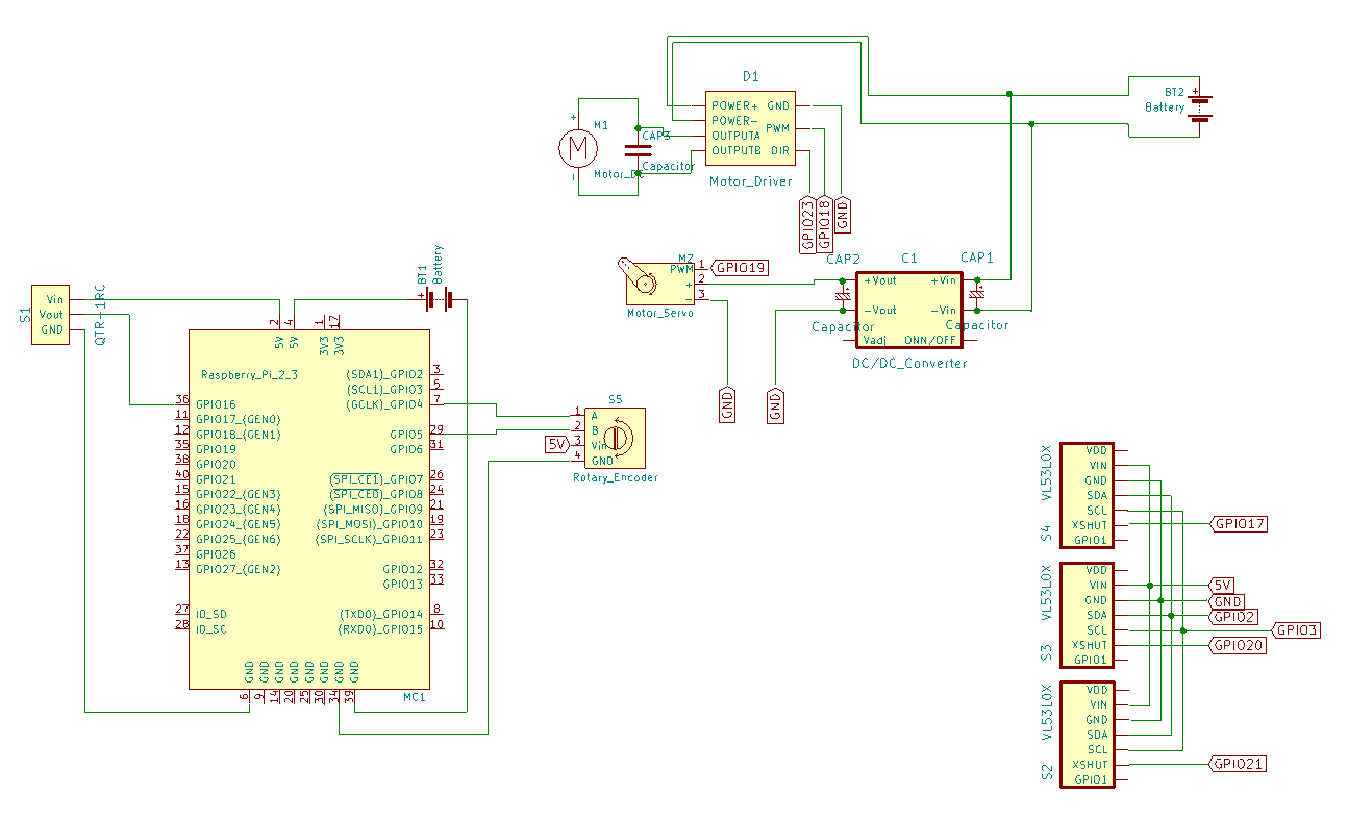
\includegraphics[scale=0.6]{picture/eps/ele_circuit_fig1.eps}
\caption{回路図}
\label{fig::overall_electric_circuit}
\end{figure}
\section{回路設計}
今回設計した回路を\refig{overall_electric_circuit},回路制作に使用した主要な部品の一覧を\reftab{circuit_parts}にそれぞれ示す.さらに各電子部品の仕様や構成について以下に示す.

\subsection{電源回路}
以下に示す仕様のようにRaspberryPi3 Model Bとサーボモータ,DCモータドライバではそれれぞれ定格電圧が異なるため同一の電源を用いることができない.そこで$7.2\unit{V}$バッテリと$5\unit{V}$バッテリの2つを用いている.
$7.2\unit{V}$バッテリはまず分流を行い,一方をDC-DCコンバータを用いて$7.2\unit{V}$から$5\unit{V}$に降圧してサーボモータに供給し,もう片方をDCモータドライバに供給している.$5\unit{V}$バッテリはRaspberryPi3 Model Bに電源を供給している.
\begin{description}
    \item[モータドライバ\textless MD10CR3\textgreater \cite{motordriver}]\mbox{}\\
    \vspace{-5mm}
        \begin{itemize}
            \item モータ電源電圧: DC $5\unit{V}-25\unit{V}$
            \item 最偉大電流  : $13\unit{A}$
            \item ロジック入力電圧: $3.3\unit{V}-5\unit{V}$
        \end{itemize}
    \item[サーボモータ\textless GWS03T/2BBMG\textgreater]\mbox{}\\
    \vspace{-5mm}
         \begin{itemize}
            \item 駆動電圧: DC $4.8\unit{V}-6\unit{V}$
        \end{itemize}
     \item[RaspberryPi3 ModelB\cite{rpi}]\mbox{}\\
     \vspace{-5mm}
         \begin{itemize}
            \item 電源: $5\unit{V}$,$2.5\unit{A}$
        \end{itemize}

\end{description}


\begin{table}
    \caption{電気回路用部品}
    \label{tab::circuit_parts}
    \begin{center}
    \footnotesize
   \begin{tabular}{ | l | l | c || l |}\hline
タイプ               &部品名                                         &数&用途   \\ \hline\hline
マイコン             &Raspberry Pi3 Model B                            &1&制御用           \\ \hline
DCモータ             &RP380-ST                                  &1&後輪モータ駆動用   \\    \hline
モータドライバ          &MD10C R3                                        &1&後輪モータ制御用   \\ \hline
距離センサ            &VL53L0X Time-of-Flight                           &3&距離計測用   \\ \hline
フォトリフレクタ         &QTR-1RC フォトリフレクタ・モジュール              &3&ゴールライン計測用   \\ \hline
DC-DCコンバータ          &BTD05-05S200D                                     &1&降圧用   \\ \hline
コンデンサ                &セラミックコンデンサ$1000\unit{pF}50\unit{V}$ &1&後輪モータのノイズ除去用   \\ \cline{2-4}
                          &OSコンデンサ $10\unit{V}47\unit{\mu F}$                          &2&DC-DCコンバータのノイズ除去用    \\ \hline
ロータリーエンコーダ   &RE30E-500-213-1                                   &1&ロボカーの速度計測用   \\ \hline
バッテリ             &Powers Max 4000 Ni-MH $7.2\unit{V}$                        &1&DCモータ,サーボモータ用の電源\\ \cline{2-4}
                          &$4000\unit{mAh}$ 6CELL ニッケル水素バッテリ                &1&Raspberry Pi3 ModelB用の電源    \\ \hline
サーボモータ           &GWS03T/2BBMG                                &1&ステアリング用   \\    \hline
 
	   \end{tabular} 
	\end{center}
\end{table}


\newpage

\begin{figure}[h!]
\centering
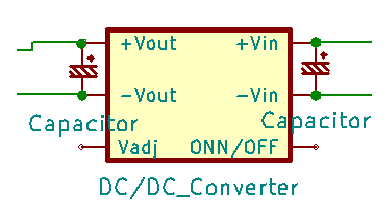
\includegraphics[scale=0.8]{picture/eps/ele_cap.eps}
\caption{DC-DCコンバータの回路図}
\label{fig::ele_cap}
\end{figure}

\subsection{DC-DCコンバータ}
本回路上で降圧を行うためにDC-DCコンバータを用いた.以下にその仕様を示す.DC-DCコンバータは内部でディジタルスイッチングを行っているため,ノイズが多い\cite{dcdc}.本回路ではこのようなノイズ成分を除去するために電解コンデンサ(OSコンデンサ$10\unit{V}47\unit{\mu F}$)を用いた\refig{ele_cap}の回路を作成した\cite{dcdcconverter}.
\begin{description}
    \item[DC-DCコンバータ\textless BTD05-05S200D\textgreater \cite{dcdcconverter}]\mbox{}\\
    \vspace{-5mm}
        \begin{itemize}
            \item 入力電圧: DC $4.5\unit{V}-9\unit{V}$
            \item 出力電圧: $0\unit{mA}-2000\unit{mA}$
            \item 出力電流: $3.3\unit{V}-5\unit{V}$
            \item 効率: 84 \%
        \end{itemize}
\end{description}


